\documentclass[output=paper]{langscibook}
\ChapterDOI{10.5281/zenodo.15006609}
\author{Allison Burkette\affiliation{University of Kentucky} and Lamont Antieau\affiliation{University of Kentucky}}
\title{Leaner, cleaner, and full of attitude}
\subtitle{The New Atlas interviews}

\abstract{Early fieldwork for the Linguistic Atlas of the United States and Canada (later, the Linguistic Atlas Project, or LAP) consisted of 6- to 8-hour-long interviews designed to elicit lexical, phonological, and grammatical targets from native informants in predominantly English-speaking communities throughout North America. Fieldworkers for the project were trained to ask questions that were usually in the form of descriptive phrases that tasked the speaker to name the item being described (these were often framed by the phrase \textit{what would you call [description]}) or fill-in-the-blank questions that asked the speaker to supply the target as the missing word (\textit{if a glass fell on a hard floor and shattered, you would say the glass \_\_\_\_\_\_}). For the earliest surveys, responses were written down in the International Phonetic Alphabet (IPA), but later interviews were tape recorded in their entirety and the responses transcribed from the recordings. The ultimate goal of the earliest surveys was the mapping of dialect boundaries, particularly the mapping of individual linguistic features.

Over time, however, the goals and structure of the LAP interview have changed. The overarching goal of LAP interviews has shifted from an interest in isoglosses and dialect boundaries to a desire to record variation and to investigate the correlations between that variation and specific social and regional groups. Today’s LAP interviews take the form of conversational interviews that still seek names for specific foods, animals, weather phenomena, etc., as well as morphological and syntactic forms, but also address the contemporary sociolinguistic interest in perceptions and attitudes. This paper provides details of the new hybrid LAP interview, one whose format offers the best of all worlds: a set of dialectological targets that will facilitate comparisons across LAP surveys and through time, the free-flowing conversation prized by traditional sociolinguistics for grammatical and phonological analysis, and questions aimed at getting at interviewees’ attitudes and beliefs about language use in their communities. Interviews have already been conducted in Kentucky with this new framework.}
\IfFileExists{../localcommands.tex}{
  \addbibresource{../localbibliography.bib}
  \usepackage{tabularx,multicol}
%\usepackage{multirow}
\usepackage{subcaption}
\usepackage{url}
\urlstyle{same}

\usepackage{datetime}
\usepackage{enumitem}
\usepackage{langsci-optional}
\usepackage{langsci-lgr}
\usepackage{langsci-branding}

\usepackage{longtable}
\usepackage{xltabular}
\usepackage[linguistics, edges]{forest}
\usepackage{pgfplots}
\pgfplotsset{compat=1.18}
\usetikzlibrary{patterns, tikzmark}
\usepackage{pgfplotstable}
\usepgfplotslibrary{colorbrewer}
\usepackage{listings}
\lstset{basicstyle=\ttfamily,keywordstyle=\normalfont,language=,breaklines=true}

\usepackage{siunitx}
\sisetup{group-digits=none, detect-all=true}

\usepackage{langsci-gb4e}

  \makeatletter
\let\thetitle\@title
\let\theauthor\@author
\makeatother

% Use this Chinese font shipped with TeX Live instead of Source Han, because
% it is more portable/leightweight. Install the "fandol" package from CTAN to
% automatically get this font.
\newfontfamily{\ChineseFandolSong}{FandolSong-Regular.otf}

  %% hyphenation points for line breaks
%% Normally, automatic hyphenation in LaTeX is very good
%% If a word is mis-hyphenated, add it to this file
%%
%% add information to TeX file before \begin{document} with:
%% %% hyphenation points for line breaks
%% Normally, automatic hyphenation in LaTeX is very good
%% If a word is mis-hyphenated, add it to this file
%%
%% add information to TeX file before \begin{document} with:
%% %% hyphenation points for line breaks
%% Normally, automatic hyphenation in LaTeX is very good
%% If a word is mis-hyphenated, add it to this file
%%
%% add information to TeX file before \begin{document} with:
%% \include{localhyphenation}
\hyphenation{
    a-na-ly-sis
    ap-proach-es
    ar-che-o-log-i-cal
    Ar-khan-gelsk
    be-schrei-ben
    Buch-holtz
    Che-lya-binsk
    con-so-nant
    dia-lect
    dia-lect-ology
    Di-a-lekt-for-schung
    Dia-lekt-for-schung
    East-pha-lian
    För-der-ung
    Ge-mein-schaft-lich-keits-ent-wür-fe
    his-tor-i-cal
    Hok-kai-do
    ja-pa-nese
    Ja-pa-nese
    Ka-go-shi-ma
    Ka-li-nin-grad
    Knja-zev
    Ma-kro-be-reich
    Ma-lay-sia
    mor-pho-log-i-cal
    Mos-cow
    Nef-te-yu-gansk
    non-mobile
    nu-cle-ar
    ös-ter-rei-chi-sche
    par-a-digm
    per-zep-ti-ons-lin-gu-is-ti-sche
    plu-ri-zen-tri-schen
    quick-ly
    Reich
    Sax-on
    Schrö-der
    sear-ching
    ste-reo-type
    strength-en-ing
    strong-est
    Stutt-gart
    su-pra-seg-men-tal
    teach-er
    to-po-gra-phy
    To-ron-to
    tra-di-tion-al
    ul-ti-mate-ly
    Um-gangs-spra-che
    Volks-kun-de
    vor-zu-stel-len
    wheth-er
    Wie-sing-er
    with-in
    Wort-at-las
}

\hyphenation{
    a-na-ly-sis
    ap-proach-es
    ar-che-o-log-i-cal
    Ar-khan-gelsk
    be-schrei-ben
    Buch-holtz
    Che-lya-binsk
    con-so-nant
    dia-lect
    dia-lect-ology
    Di-a-lekt-for-schung
    Dia-lekt-for-schung
    East-pha-lian
    För-der-ung
    Ge-mein-schaft-lich-keits-ent-wür-fe
    his-tor-i-cal
    Hok-kai-do
    ja-pa-nese
    Ja-pa-nese
    Ka-go-shi-ma
    Ka-li-nin-grad
    Knja-zev
    Ma-kro-be-reich
    Ma-lay-sia
    mor-pho-log-i-cal
    Mos-cow
    Nef-te-yu-gansk
    non-mobile
    nu-cle-ar
    ös-ter-rei-chi-sche
    par-a-digm
    per-zep-ti-ons-lin-gu-is-ti-sche
    plu-ri-zen-tri-schen
    quick-ly
    Reich
    Sax-on
    Schrö-der
    sear-ching
    ste-reo-type
    strength-en-ing
    strong-est
    Stutt-gart
    su-pra-seg-men-tal
    teach-er
    to-po-gra-phy
    To-ron-to
    tra-di-tion-al
    ul-ti-mate-ly
    Um-gangs-spra-che
    Volks-kun-de
    vor-zu-stel-len
    wheth-er
    Wie-sing-er
    with-in
    Wort-at-las
}

\hyphenation{
    a-na-ly-sis
    ap-proach-es
    ar-che-o-log-i-cal
    Ar-khan-gelsk
    be-schrei-ben
    Buch-holtz
    Che-lya-binsk
    con-so-nant
    dia-lect
    dia-lect-ology
    Di-a-lekt-for-schung
    Dia-lekt-for-schung
    East-pha-lian
    För-der-ung
    Ge-mein-schaft-lich-keits-ent-wür-fe
    his-tor-i-cal
    Hok-kai-do
    ja-pa-nese
    Ja-pa-nese
    Ka-go-shi-ma
    Ka-li-nin-grad
    Knja-zev
    Ma-kro-be-reich
    Ma-lay-sia
    mor-pho-log-i-cal
    Mos-cow
    Nef-te-yu-gansk
    non-mobile
    nu-cle-ar
    ös-ter-rei-chi-sche
    par-a-digm
    per-zep-ti-ons-lin-gu-is-ti-sche
    plu-ri-zen-tri-schen
    quick-ly
    Reich
    Sax-on
    Schrö-der
    sear-ching
    ste-reo-type
    strength-en-ing
    strong-est
    Stutt-gart
    su-pra-seg-men-tal
    teach-er
    to-po-gra-phy
    To-ron-to
    tra-di-tion-al
    ul-ti-mate-ly
    Um-gangs-spra-che
    Volks-kun-de
    vor-zu-stel-len
    wheth-er
    Wie-sing-er
    with-in
    Wort-at-las
}

  \togglepaper[1]%%chapternumber
}{}

\begin{document}
\maketitle
\label{chap:burkette}
\graphicspath{{figures/burkette}}
\shorttitlerunninghead{Leaner, cleaner, and full of attitude}%%use this for an abridged title in the page headers

\section{Opening remarks}
\label{sec:burkette:1}

In this paper, we describe current efforts at the University of Kentucky to adapt traditional Linguistic Atlas Project (LAP) methods to reflect a new generation of speakers and technology and to attract a new generation of students and future researchers. As an important part of this investigation, we aim to produce results that are comparable with those collected by earlier LAP projects, so one of our tasks has been to place all results on a similar digital playing field. This has entailed organizing and cataloging many kinds of older LAP materials (e.g., paper, recordings of various media types, transcriptions, etc.) and digitizing that which had not previously been digitized at the University of Georgia. This massive endeavor was fueled by the desire to make LAP materials more accessible to researchers in dialectology and sociolinguistics who are interested in studying language variation and change.

Just as importantly, if not more so, we wish to encourage students to become interested in and engaged in all aspects of the collection and preservation of LAP data, including fieldwork, thus continuing the tradition of using the LAP as a laboratory for new and future linguists. The motivation for doing so is grounded in the belief that the best way to learn how to do something is through hands-on, practical experience (and the belief that to know the Atlas is to love the Atlas).  

\section{Background} %2
\label{sec:burkette:2}
\subsection{The Linguistic Atlas Project} %2.1
\label{sec:burkette:2.1}
\largerpage
The LAP began in 1929 when Hans Kurath was asked by the American Dialect Society to undertake a large-scale survey of American English. Kurath began training fieldworkers in 1930 and with them began the systematic investigation of variation in regional American English. Fieldwork began with the Linguistic Atlas of New England (LANE) in 1931, which was then followed by the Linguistic Atlas of the Middle and South Atlantic States (LAMSAS), and the Linguistic Atlas of the North Central States (LANCS). These early LAP surveys employed face-to-face interviews to elicit speakers’ responses to a lengthy questionnaire that contained over 800 prompts aimed at capturing variation in regional vocabulary, pronunciation, and grammar. The bulk of these early interviews took the form of questions aimed at eliciting specific responses, such as \textit{what do you call [description]} or fill-in-the-blank questions that asked the speaker to supply the target as the missing word (\textit{if a glass fell on a hard floor and shattered, you would say the glass \_\_\_\_}). We know now, however, that many fieldworkers also integrated more conversational prompts into the interviews, such as \textit{tell me about \_\_\_\_}, which prompted longer, sometimes narrative, answers. Although a smattering of brief recordings exists from these early surveys, the main mode of data collection took the form of on-the-spot, handwritten International Phonetic Alphabet transcription of words or phrases. These transcriptions, collectively referred to as field pages, have been the main source of data for most of the LAP studies carried out to date. 

Data collection for the LAP has never been a linear process; the bulk of the LAMSAS interviews took place in the 1930s and '40s and the bulk of LANCS interviews in the 1950s and '60s, but there were other surveys being conducted concurrently, such as the interviews with Gullah speakers conducted by Lorenzo Dow Turner in 1933 and the Linguistic Atlas of Hawai’i (LAH), directed by C.M. Wise during his year as a visiting professor at the University of Hawaii in 1950. 

Historically, the aim of the LAP interview was, as \citet[13]{Kurath1972} put it, to collect ``the speechways of the folk'', with the ultimate goal of the earliest surveys being the delineation of dialect boundaries, an exercise interwoven with the creation of maps of individual linguistic features. Over time, however, the goals and structure of the interview have changed. The overarching goal of LAP interviews has shifted from an interest in isoglosses and dialect boundaries to a desire to record variation and to look at the correlations between that variation and specific social and regional groups. Starting in the late 1960s with the Linguistic Atlas of the Gulf States (LAGS), LAP fieldworkers under the direction of Lee Pederson implemented an interview structure that encouraged a more conversational exchange.

With LAGS in the process of publication \citep{PedersonCarolAdams1986}, Pederson set his sights on bringing together existing LAP databases from across the continent while also surveying large parts of the western United States that had not been previously covered by earlier fieldwork \citep{Pederson1996b}. As part of Pederson’s plan for the project \citep{Pederson1990}, fieldworkers would tape-record three-hour interviews with natives of communities in the West in their entirety. These recordings would then be transcribed in more or less standard orthography, thus allowing for the interviews to be processed using digital tools to compile wordlists, to get wordcounts, to investigate keywords in context, and the like. To this end, he sought to make interviews much shorter (down to 360 targets over the course of three hours) while still ensuring they would be largely comparable to earlier interviews in terms of lexical and phonetic targets. Prompts for the grammatical features that had been targeted by earlier worksheets were eliminated, and instead the worksheets placed greater emphasis on conversation from which grammatical variants might emerge more naturally. Additionally, some of the tasks/targets that might make informants self-conscious, such as counting and providing the names of days and months, as well as names for body parts, were moved to late in the interviews. Finally, there was a focus in the interviews on the language and culture of the Western states.

Fieldwork for the Linguistic Atlas of the Western States (LAWS) began with interviews of 15 native informants in Wyoming in 1988 (\citealt{PedersonMadsen1989}), before fieldwork commenced in Colorado and Utah for a Linguistic Atlas of the Middle Rockies (LAMR: \citealt{Pederson1996b, Antieau2012, AntieauDarwin2013}), as well as El Paso, Texas \citep{Hamilton-Brehm2003}, and southern California. Pederson then went on to use the same methods in his fieldwork in the Caribbean islands of St. Kitts and Nevis (\citealt{BakerPederson2013}). 

While many basic assumptions and methods of the LAP have remained constant through the years, in part to ensure that more recently collected data is comparable to the earliest LAP data, LAP methodology has evolved in several ways. For instance, while the earliest LAP components often sought nonmobile, older, rural males (NORMs) for interviews, there has been some effort to make the informant pool more inclusive with regard to the sex of the informant, their education level, profession, etc. NORMs also tended to be white, and LAGS, in particular, made an effort to have a more balanced representation with respect to race. While the LANE and LAMSAS informant pools evidence a gross underrepresentation of women and people of color, LAGS informants were chosen in a more demographically representative manner. For example, LANE had two African American informants (out of 416 informants total) and LAMSAS had 41 (out of 1162), but LAGS contains data from 241 African American speakers (out of 914). 

The process of audio recording was integrated into LAP interviewing early on, albeit sporadically and not exhaustively, and continued to varying extents in many of the subsequent LAP components, but the tools for recording and the motivation for doing so have changed over time. In 1940, LANE collected speech samples from over 400 informants in the field on machines capable of recording to aluminum disk at 78 rpm. These disks are stored at the Special Collections Library at the University of Kentucky, with copies at the Library of Congress, where digital copies are also archived. For the Linguistic Atlas of the Upper Midwest (LAUM), Allen collected speech samples of many of his informants \citep[2--3]{Allen1973} on wire and tape.{\interfootnotelinepenalty=10000\footnote{Unfortunately, the location of the disks that Allen’s wire and tape recordings were transferred to has been unknown for quite some time, and although four of Allen’s wire recordings apparently existed in 1967, wire is considered to be an unstable and, hence, temporary audio-recording format (\citealt[32--33]{Howren1967}). Furthermore, none of these recordings and/or copies are in the current LAP inventory.}} Some interviews conducted for LAMSAS and LANCS, as well as the Linguistic Atlas of the Pacific Northwest (LAPNW), were recorded using reel-to-reel tape; these tapes are located at the University of Kentucky, and many have already been digitized. All Linguistic Atlas of Oklahoma (LAO) and LAGS interviews were recorded in their entirety on reel-to-reel tape, thus replacing the phonetic transcription in the field that up until then had always been the primary method of recording data. The targets on these tapes were later transcribed on paper. LAGS tapes, as well as digitized LAO and LAGS recordings, are housed at the University of Kentucky. LAWS interviews were taped on audio cassette, and both the cassettes and the digitized files are archived at the University of Kentucky. Finally, the digitized interviews from St. Kitts and Nevis are also stored at the University of Kentucky.

\section{The New Atlas Interviews} % 3.
\label{sec:burkette:3}
\subsection{Motivation for the work} % 3.1. /
\label{sec:burkette:3.1}
The main goal of today’s LAP team is threefold. We want to make the historical LAP data available and accessible online for researchers and other interested parties. For researchers in sociolinguistics, specifically, we want to demonstrate that the LAP data can offer the best of all worlds: a set of dialectological targets that will facilitate comparisons across the LAP surveys and through time, the free-flowing conversation prized by traditional sociolinguistics for grammatical and phonological analysis, and a task that will elicit interviewees’ language regard factors about language use in the area (see \citealt{Preston2018, Preston2019}). And finally, today’s LAP still hopes to collect the “speechways of the folk'' but wants to make sure that all folk are represented.

Much of what we intend to do in Kentucky adheres to the framework of the most recent of the major LAP components, LAWS, in that we aim to audio record interviews with native informants in their entirety, transcribe the interviews, and rely on the resulting transcriptions as the primary data for analysis. At the same time, we want to incorporate advancements in recording that have occurred since the creation of the LAWS project in the late 1980s – notably, being able to record straight to digital in the field – and thus eliminate the need for digitization after the fact, freeing up time for other tasks.

\subsection{Grid units} % 3.2.
\label{sec:burkette:3.2}

Since an important aspect of this new work is to produce data that is comparable to older LAP data, using the same grid units established by the LAP for earlier work (in areas where earlier work was done) is appropriate, barring any significant changes in the political boundaries (such as state and county lines) of that region. (For more on grid units in LAP, see, e.g., \cites[39--40]{Kurath1973}[23--24]{Allen1973}[4]{Pederson1990}) This will allow for real-time studies in the spirit of \citegen{Johnson1996} work using LAMSAS interviews conducted in the states of Georgia and North and South Carolina in 1930 and her own follow-up interviews in those same states in 1990. Because the state of Kentucky and its political boundaries have not undergone a major shift since fieldwork was conducted in the mid-20\textsuperscript{th} century as part of the LANCS project, we are using the same ones established in the state for that project.

\subsection{The perceptual component} %3.3
\label{sec:burkette:3.3}
Attention to language regard entails the collection and study of attitudinal data that contribute to our understanding of the viewpoints, beliefs, and ideologies that people have about language and language use (\citealt{Preston2018, Preston2019}). Although aspects of regard have not before been sought in most LAP work, our work in Kentucky will address regard directly. The goal of incorporating interview techniques from perceptual dialectology, such as the draw-a-map task, into the new LAP interview is to trigger conversational data that serendipitously contains explicit and implicit clues to language regard.

\begin{figure}
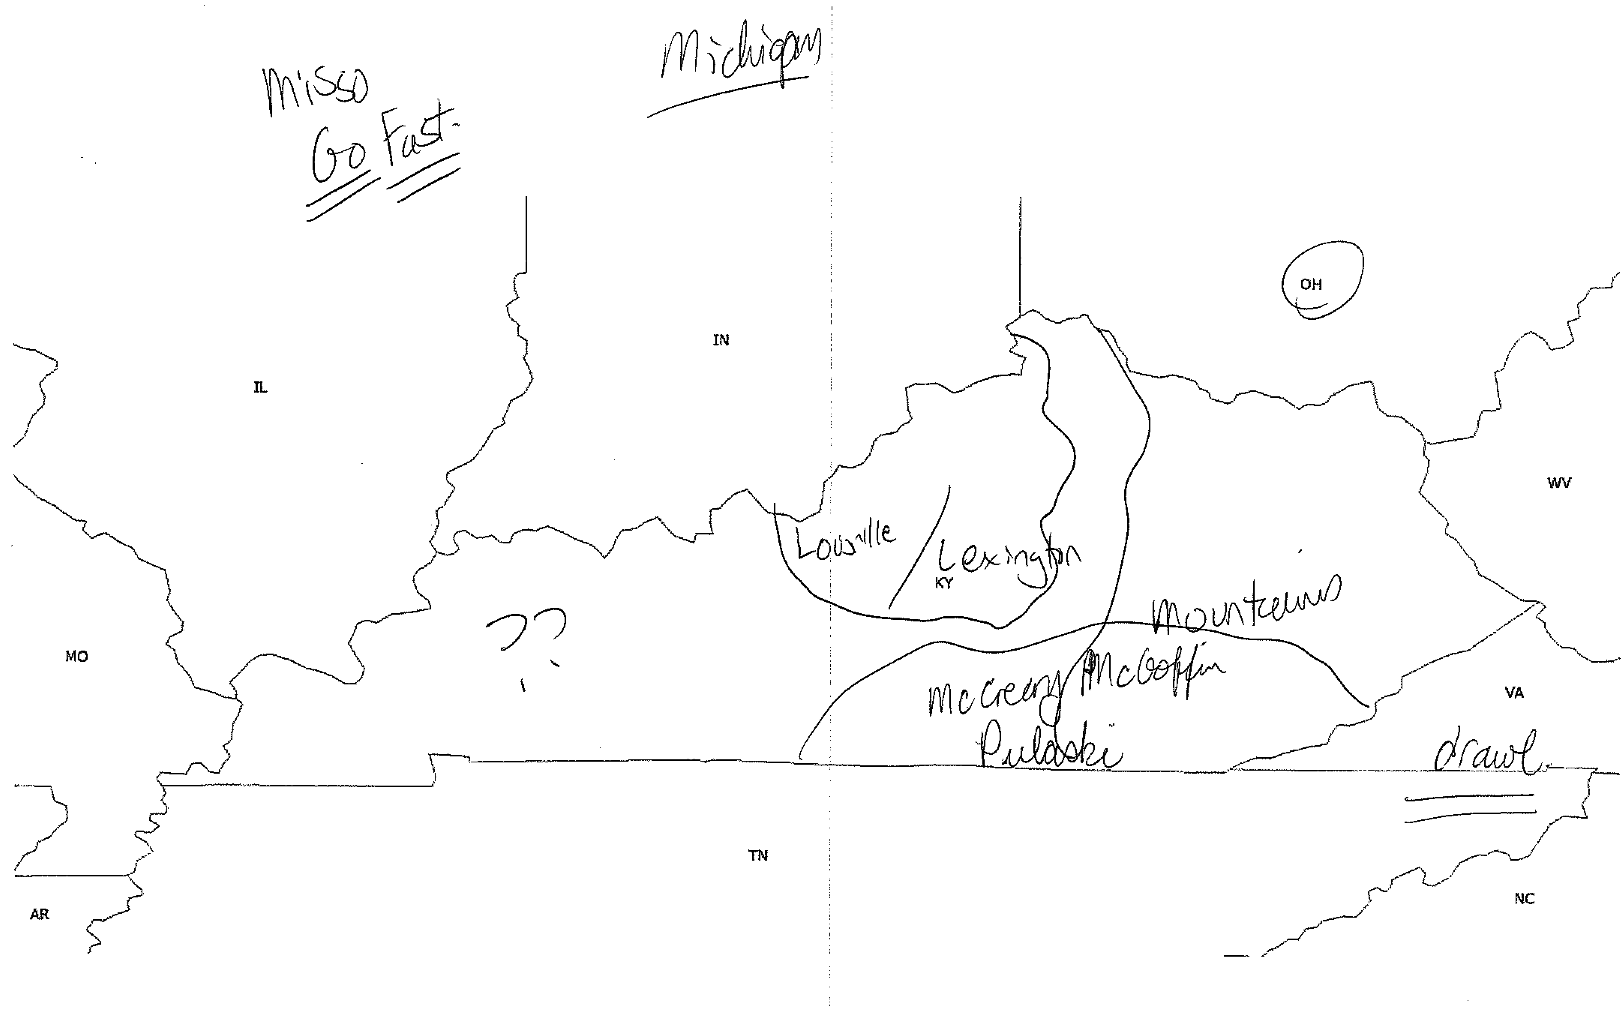
\includegraphics[width=\textwidth]{burkette-img001.pdf}
\caption{\label{fig:burkette:1}Hand-drawn perceptual dialectology map of a 66-year-old white female Louisville respondent from 2022.}
\end{figure}

The extended conversations from the map-drawing task as well as other interactions that may arise will offer many opportunities to report and analyze language regard issues. Recent work in anthropological and semanto-pragmatic approaches to conversational data also suggest that implicit regard factors may be extracted from data in this way. \citet[25]{Irvine2001} explains: ``the best place to look for language ideology may lie in the terms and presuppositions of metapragmatic discourse, not just in its assertions''. We have already piloted such analytic approaches, even with older LANCS data (\citealt{George2022, Passarelli2023}) and are convinced that we will encounter not only valuable overt assertions about language regard but also will find many opportunities to look at implicit or nonasserted material found in both semantic and pragmatic presuppositions and implicatures (\citealt{Preston2019,Preston2023}).

\subsection{Community and informant selection} % 3.4, not 3.3
\label{sec:burkette:3.4}
Along the same lines, the communities surveyed for earlier projects should be considered as locations for new interviewing, although communities that are close in proximity and character to the original communities will serve as well. Some of the communities that were sites of earlier LAP interviews no longer exist, sometimes only in name but other times as distinct political entities, having been absorbed by neighboring towns or cities, or becoming ghost towns through population loss, often as a result of the depletion or devaluation of the economic attraction that brought people there in the first place. Such situations obviously require the use of another community within the established grid unit for fieldwork. 

With respect to informant selection, finding new informants based on their sharing similar demographic characteristics with earlier informants might be ideal for focusing only on linguistic change; however, our interest in language variation and in the LAP being representative of more diverse populations of communities is at odds with a methodology that tended to seek out NORMs, or at least elderly informants, for interviewing. We are also aware that students, especially those whose major interest in conducting an Atlas interview is for course credit, tend to not wander outside their comfort zone and instead lean on family and friends for the purposes of their interview. Thus, at this point we are mainly interested in informants who identify as natives of the communities they represent; older informants are preferred but not required, and informants with some knowledge of farming (or ranching, depending on the location) terminology are also desired, as the worksheets include many such terms.   

In \figref{fig:burkette:2}, the primary area where we have conducted and will continue to conduct new interviews is indicated by shading. Thus far, most of the new interviews have been conducted with speakers from Kentucky’s two largest cities, Louisville and Lexington.

\begin{figure}
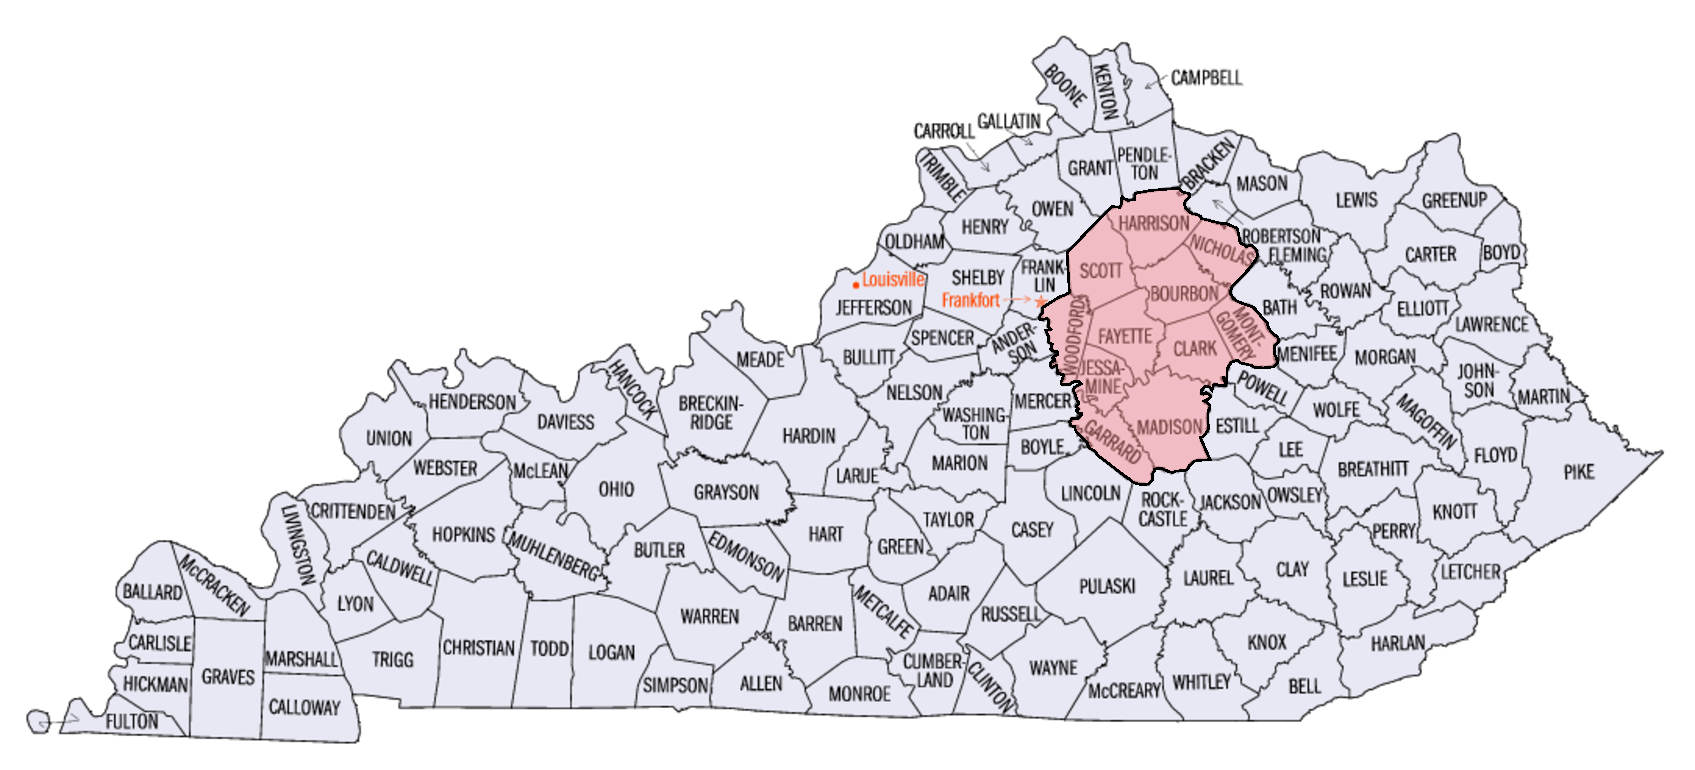
\includegraphics[width=\textwidth]{burkette-img002_2.pdf}
\caption{\label{fig:burkette:2}Primary area of focus for new Kentucky interviews. Original map from \url{https://commons.wikimedia.org/wiki/File:Kentucky_counties_map.gif}.}
\end{figure}

\subsection{Worksheets} %3.5, not 3.4
\label{sec:burkette:3.5}
In that they play a pivotal role in any LAP investigation, we have extensively reviewed previous LAP worksheets to create the best worksheets possible for conducting the new Atlas interviews. In addition to the LANE worksheets, from which all LAP worksheets have been derived, the new Kentucky worksheets are a blend of two sets of worksheets in particular: LANCS and LAWS. More specifically, our aim is to collect data largely comparable to that collected in the LANCS fieldwork in Kentucky in the mid-20\textsuperscript{th} century so we can look at linguistic change. At the same time, we want worksheets that will create a comfortable situation for fieldworker and informant alike, an environment in which the speech that is elicited not only yields lexical and phonological data comparable to earlier data but that can be used for syntactic and even pragmatic analysis as well. Additionally, we want to take advantage of this opportunity to incorporate a new component not previously dealt with explicitly in LAP interviews: data for perceptual dialectology (\citealt{Preston2018, Preston2019}).

We began our creation of the new Kentucky worksheets with the LAWS worksheets \citep{Pederson1996a} as our base because of those worksheets being intended for shorter interviews that did not directly target grammatical features, for the most part, and in fact tried to delay the questions that might make speakers self-conscious, such as counting and reciting days of the year, names for parts of the body, and labels for different social categories, until later in the interview. The 12 semantic domains of the LAWS worksheets align with our own interests in such things as the vocabulary of house design and construction, as well as furnishings, kinship terminology, flora and fauna, and weather terms, although Pederson’s motivation for the number and size of these domains (three domains per each side of two 90-minute cassettes) no longer rigidly applies to the digital recording we will be doing, which is discussed further below. 

At the same time, some changes have been made to the LAWS format for new Kentucky fieldwork. First, some of the items that were appropriate for fieldwork in the West, such as geographical and weather-related differences unique to that region, were replaced by items more suitable to life in the Bluegrass State, many of which came from the LANCS worksheets. Worksheets will continue to be refined as we conduct interviews and find questions that yield nothing of interest or where we find evidence of new forms that we want to elicit. 

Additionally, Pederson introduced a task to LAWS interviewing whereby an informant was handed pictures of a saddle and bridle and asked to name their parts. Although this activity experienced only limited success in Rocky Mountain fieldwork, there is enough interest in horses in various parts of Kentucky to suggest that continuing to perform such a task might be worthy of consideration. 

We have continued Pederson’s work of streamlining worksheets to the amount of information that can be elicited in the shortest amount of time possible and to strive for the least self-conscious speech possible while at the same time reducing the workload back in the Atlas office so that interviews can be made available to researchers more quickly. For instance, the first page of the LAWS worksheets asked for several pieces of information -- most notably, the names of informants and their addresses -- that hold questionable value for the interview and were probably only there for logistical reasons that can be, and, at least since the second author’s fieldwork in Colorado in 2001--2004, have been collected by other and better means (most notably in the mandatory collection of signed human subject consent forms). This information was redacted in transcription and in the digitization of taped interviews before being posted for the public anyway. Thus, the current practice eschews asking informants for such information and only asks them for their zip code, as it establishes some idea of place and holds value in terms of the pronunciation of numbers.  

The LAWS worksheets have some issues of redundancy and the potential to lead informants at the beginning of the interview, specifically on the first page, between the gathering of logistical information and the elicitation of targets in the first semantic domain. For instance, following the LAWS worksheets, a fieldworker asks for information about various members of the family, such as what their relationship was to the informant (e.g. mother, father, sister, brother), where they were born, and how they made their living, before going on to other biographical information pertaining to the informants, such as the schools they attended, their own profession, groups they were part of, etc. Then, the linguistic elicitation begins, with the first semantic domain targeting words for family, education, church, etc. The current worksheets instead integrate the gathering of both types of data with the use of an early \textit{shotgun} prompt: \textit{Tell me about your family growing up}. In this way, the terms informants used for family members can be elicited more organically and avoids the priming that might otherwise occur (e.g. \textit{what did you call your mother growing up}?), while also leaving room for follow-up prompts for specific targets that the informant may not have used in their initial response (e.g. \textit{you mentioned your mother; did you have other terms for her growing up?}).     

As this will typically be the first, and oftentimes only, LAP interview that students will have the opportunity to conduct, as well as the fact that the worksheets include targets that may be unfamiliar to some if not all of these students, a sheet of fully formed questions for eliciting targets has been compiled and is being made available to fieldworkers, to be used in preparation for interviewing and/or used as an aid in the interview when fieldworkers encounter difficulty articulating a prompt on the fly. However, too much reliance on these questions might cause informants to shift from the conversational tone being sought for these interviews to a more formal manner; thus, we stress that fieldworkers should rely on these questions only as a very last resort. 

Finally, we recently began to integrate a perceptual component to the LAP interview by engaging informants in the draw-a-map perceptual dialectology task, a technique already carried out in Kentucky by \citet{Cramer2016}. In this task, respondents are given a blank map of Kentucky and asked to 1) outline the areas where people speak differently, and 2) write in examples of and comments on the speech and identities of the people in the outlined regions. (See \figref{fig:burkette:1} above for an example of a completed map.) Although these data may be treated independently in the perceptual dialectological tradition (e.g., \citealt{Preston2010}), the primary use of the technique here is to trigger conversational data that serendipitously contains explicit and implicit clues to language regard. The pragmatic and discourse\slash conversation\hyp analytic techniques outlined in \citet{NiedzielskiPreston2003} and \citet{Preston2019} will allow us to interpret what our respondents say about all aspects of language, particularly, of course, their own language use and its contrast with others. This aspect of the new LAP interview will provide a broader and more in-depth look at language regard than is normally expressed in short-term language surveys and is an important characteristic of variationist interests in language change. 

\subsection{Audio recording} % 3.6, not 3.5
\label{sec:burkette:3.6}
As mentioned above, various components of the LAP used available means of audio recording to document at least parts of interviews. Digitizing these analog artifacts has been a focus of the LAP for many years and continues to be so. It is important to note at this time that the LAP has six recordings from Kentucky in its holdings, although the quality of the recordings in terms of both listenability and completeness of interview has yet to be determined.

With respect to the new Atlas interviews, at least for the work being done in Kentucky, several methods of recording the interviews were considered. These typically implemented a combination of iPad, audio interface, lightning adapter, and microphone that required phantom power. However, these configurations were assessed as being less than ideal for interviews taking place out of controlled settings, vulnerable in a number of ways to the types of failures that have been an issue in previous LAP recording using simpler setups, and possibly harmful to the casual tone being sought in these interviews. We eventually settled on a configuration that consisted simply of an external microphone (Shure MV188 IOS Digital Stereo Condenser Microphone) that could be plugged directly into an iPad or iPhone, either that the students owned or that could be borrowed from the LAP office. In testing this configuration in the office, the resulting file provided high-quality sound, while also allowing us to bypass the time-consuming digitization process required for older analog recordings of, e.g., the LAGS and LAWS interviews, by going straight to digital. 

\subsection{Processing and analytical tools} % 3.7, not 3.6
\label{sec:burkette:3.7}

Since the advent of the LAWS project near the end of the 1980s, the end-product of LAP interviews has been an audio recording of the interviews in their entirety. This is followed by transcription of the recording in its entirety in standard orthography in machine-readable text, which can subsequently be processed by computational tools such as AntConc or KwicKwic. The finished transcript can also be used as a guide for finding select features in the audio recordings or simply read by the interested party. The 70 transcriptions of the LAMR recordings were done by Pederson and Antieau, and scribes under their direction, and later edited by Antieau. We are now investigating the use of software to create transcriptions of earlier LAP recordings, e.g. those collected for the LAGS and LAO components, followed by human editing of the manuscripts. As the new Atlas interviews will also be recorded in their entirety, such tools will also be useful for creating transcripts and compiling a corpus of the collected interview transcripts.

\section{Discussion} % 4
\label{sec:burkette:4}
\subsection{The initial new Kentucky interview} % 4.1.
\label{sec:burkette:4.1}
The first of the new Kentucky interviews was conducted by the second author of this chapter in  {July 2021}. The informant was found through the friend-of-a-friend approach; he was a 92-year-old man who was born in Louisville, Kentucky, but considered Lexington his home since his acceptance at the University of Kentucky, where he earned a degree in engineering. After graduation, he found a job with a Lexington company building roads throughout the Mid-Atlantic and Southeastern regions of the United States. He eventually established his own road construction business in Lexington and continued to do this work throughout the region. By the time of the interview, he had sold his business and retired. The three-hour interview was conducted in the informant’s Lexington home, and the fieldworker implemented the revised worksheets and the audio recording configuration described above.

The interview presented no major issues, although the recording has not yet been transcribed in its entirety. The fieldworker had never worked in the area of perceptual dialectology, so he was apprehensive about broaching the subject with the informant and presenting the map for illustrating his perceptions of the speech of people throughout Kentucky and in the surrounding environs, as this task presents itself as a departure from the prompt-response format of most of the interview. However, the informant took to the task immediately, marking areas where he thought people in the surrounding region talked differently than Lexington inhabitants and telling why he believed so (aided greatly by his travel for work throughout the region).

\subsection{Subsequent interviews} %4.2.
\label{sec:burkette:4.2}
Subsequent interviews have been conducted by students as part of an effort to both expand the present-day informant pool and to develop training materials that could be used by researchers interested in contributing to the LAP. Eight interviews with speakers in Lexington and Louisville were conducted by graduate students, and four interviews with speakers from three counties in western Kentucky were conducted by a single undergraduate. The transition to a hybrid interview format has also signaled a technological transition. The LAP has traditionally been heavily dependent on an overabundance of paper. Student interviewees were encouraged to experiment with different means of deploying the new LAP worksheets in the field, with most opting against printed worksheets in favor of digital ones. 

The images in \figref{fig:burkette:3} are an example of how one student used digital worksheets on a tablet as a way for keeping track of what was occurring in the interview. The student used color coding to note information such as what questions were asked and answered/not answered as well as what subjects were unfamiliar to the speaker. The goal now is to test various means of note-taking and digital map-drawing in the hopes of developing a uniform system that can be included in our training materials and then employed in future interviews.     

\vfill
\begin{figure}[H]
\begin{minipage}{0.5\textwidth}
% 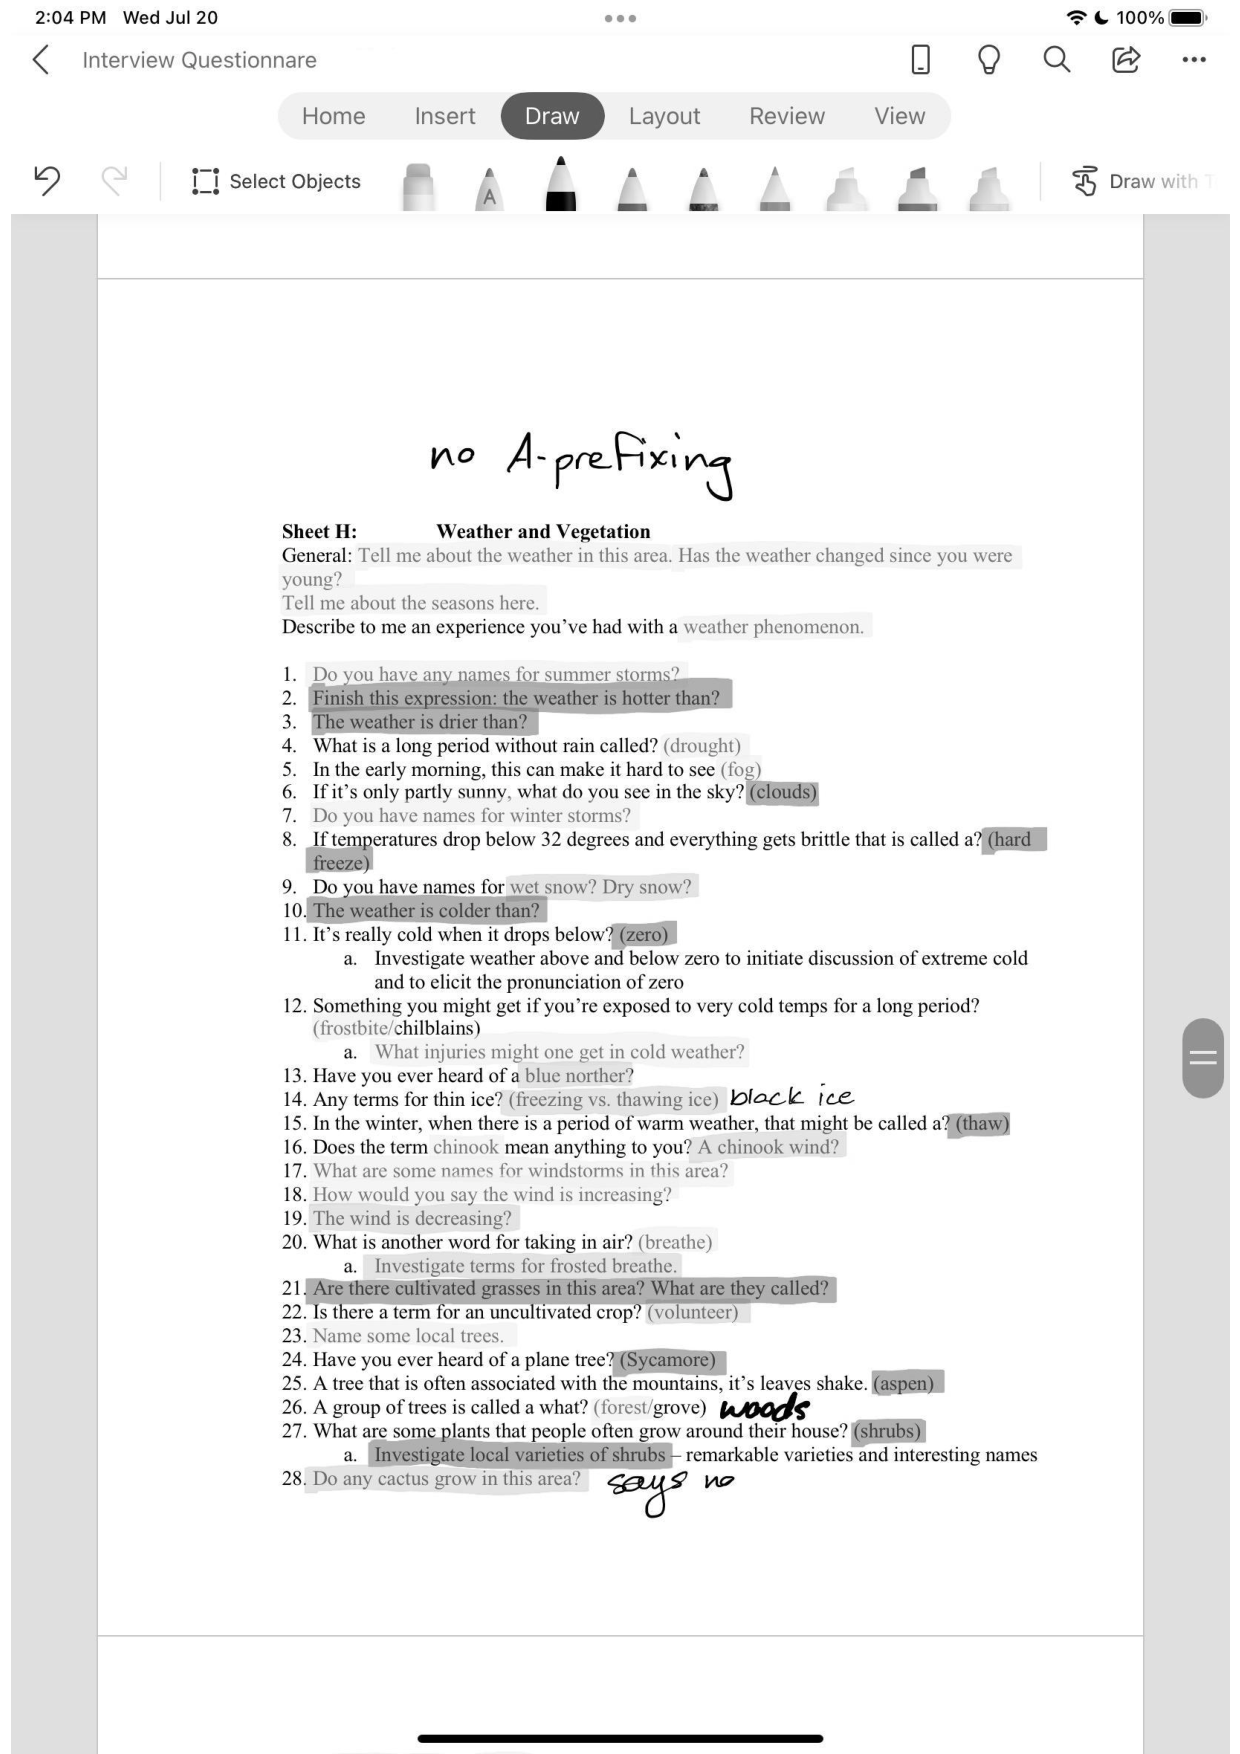
\includegraphics[width=.6\textwidth]{burkette-img003a-bw.pdf}
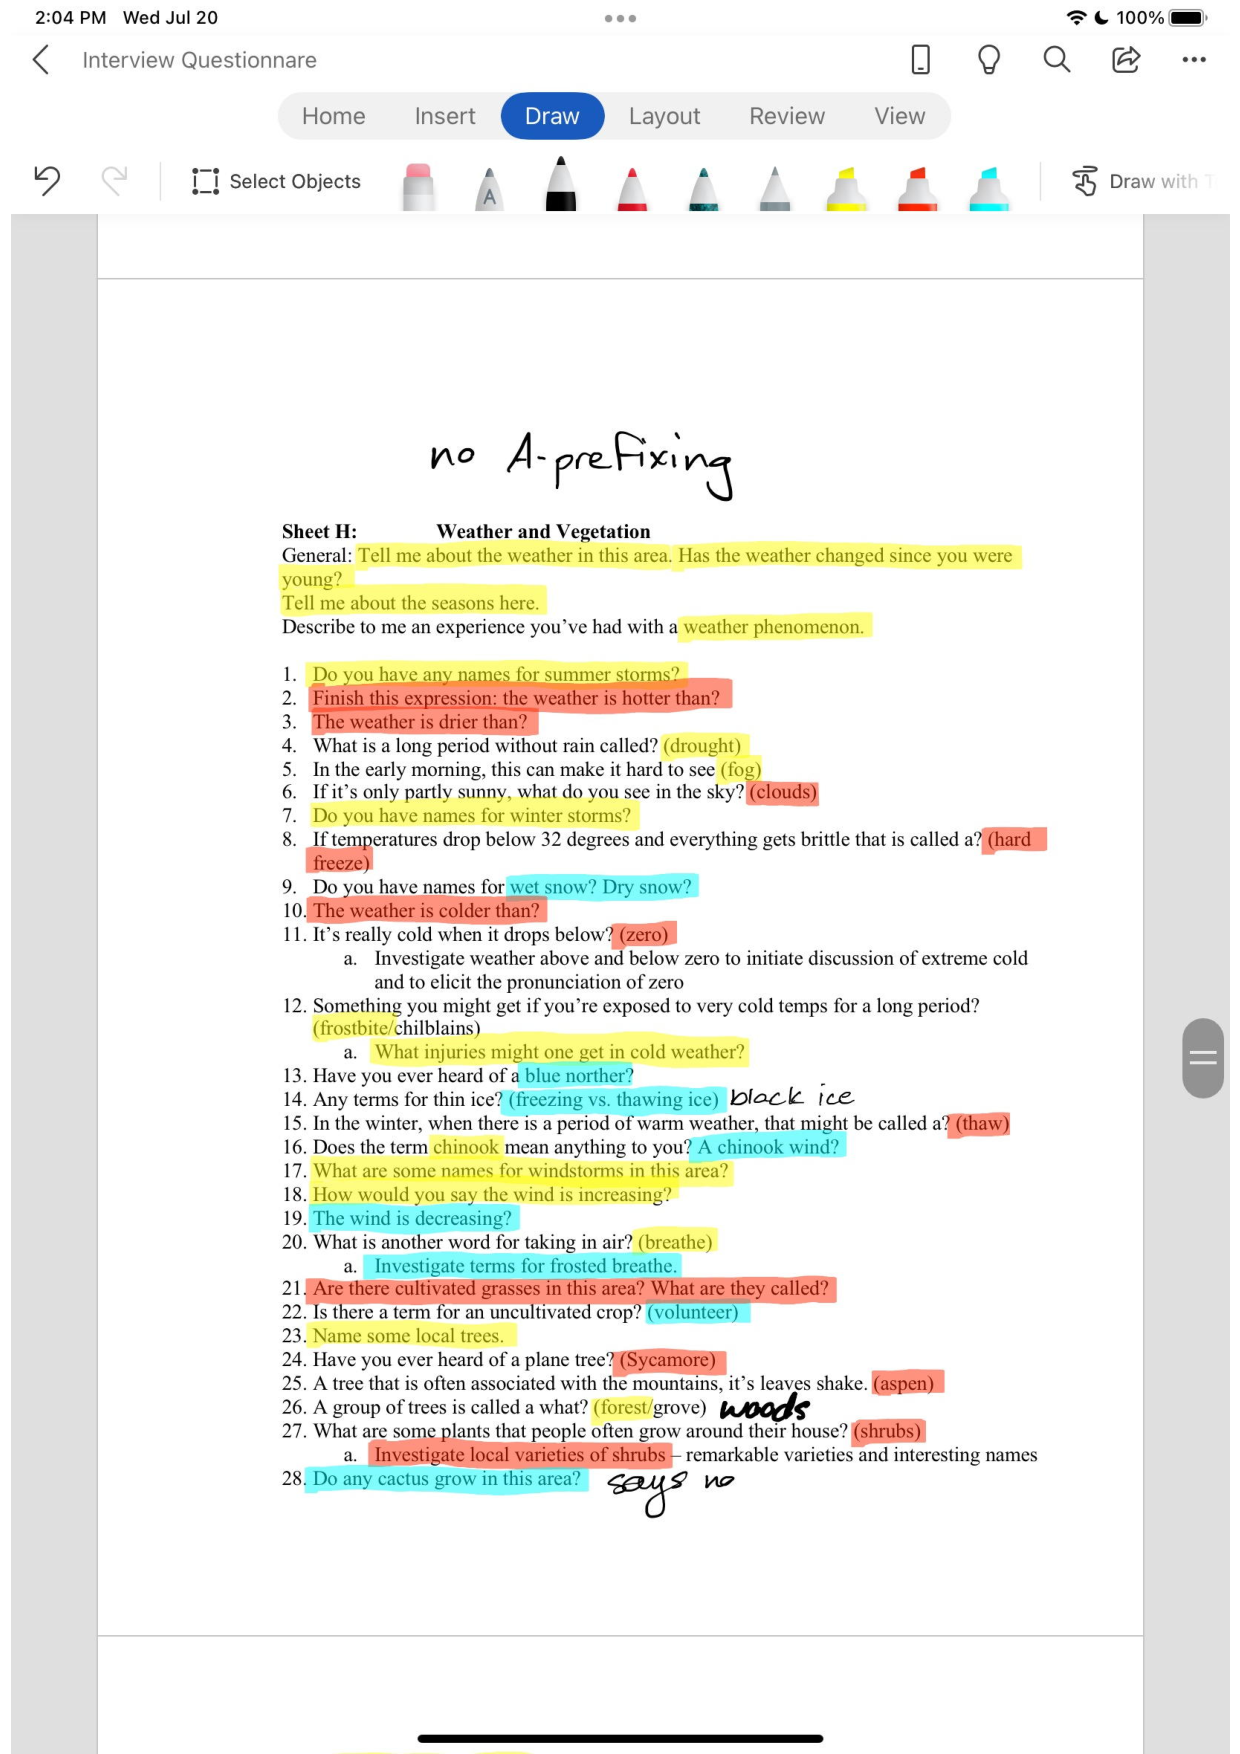
\includegraphics[width=\textwidth]{burkette-img003a-color.pdf}
\end{minipage}%
\begin{minipage}{0.5\textwidth}
% 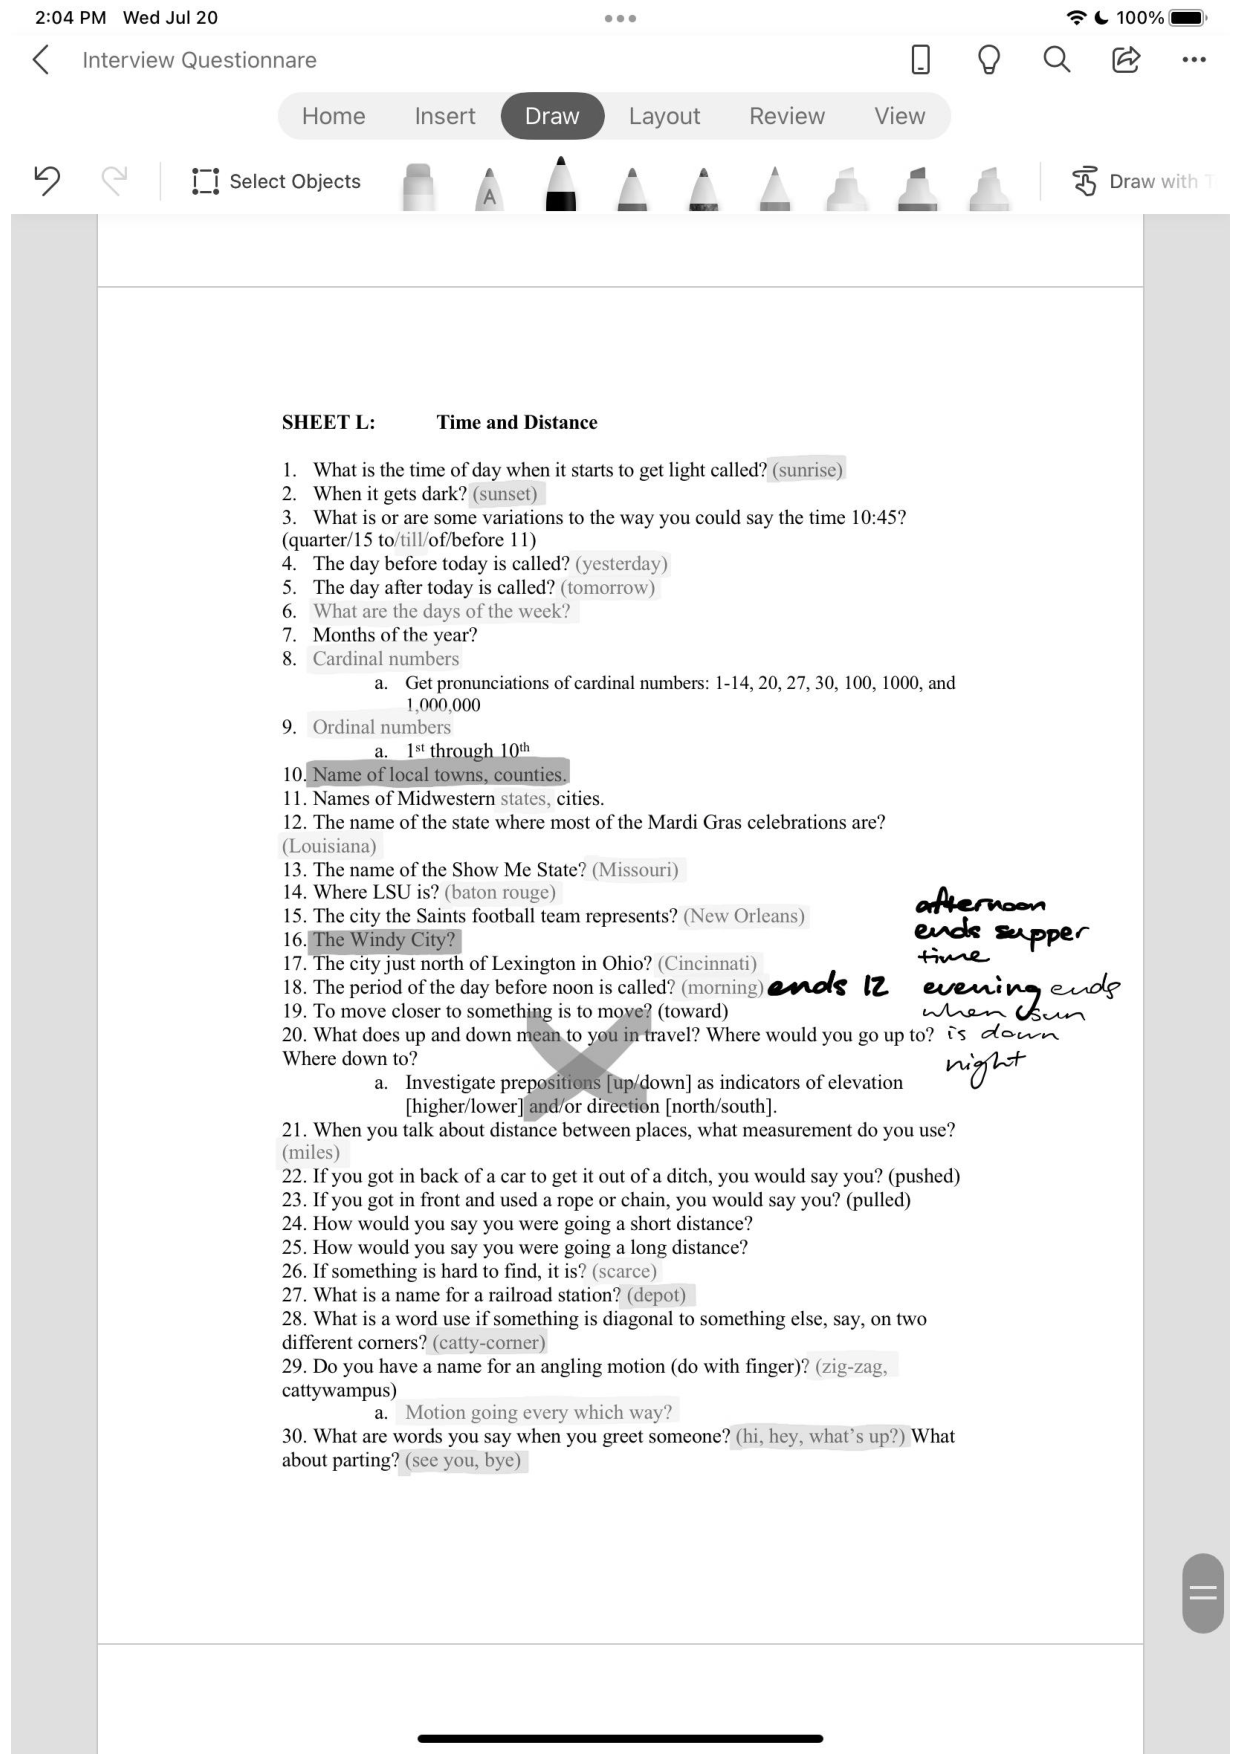
\includegraphics[width=.6\textwidth]{burkette-img003b-bw.pdf}
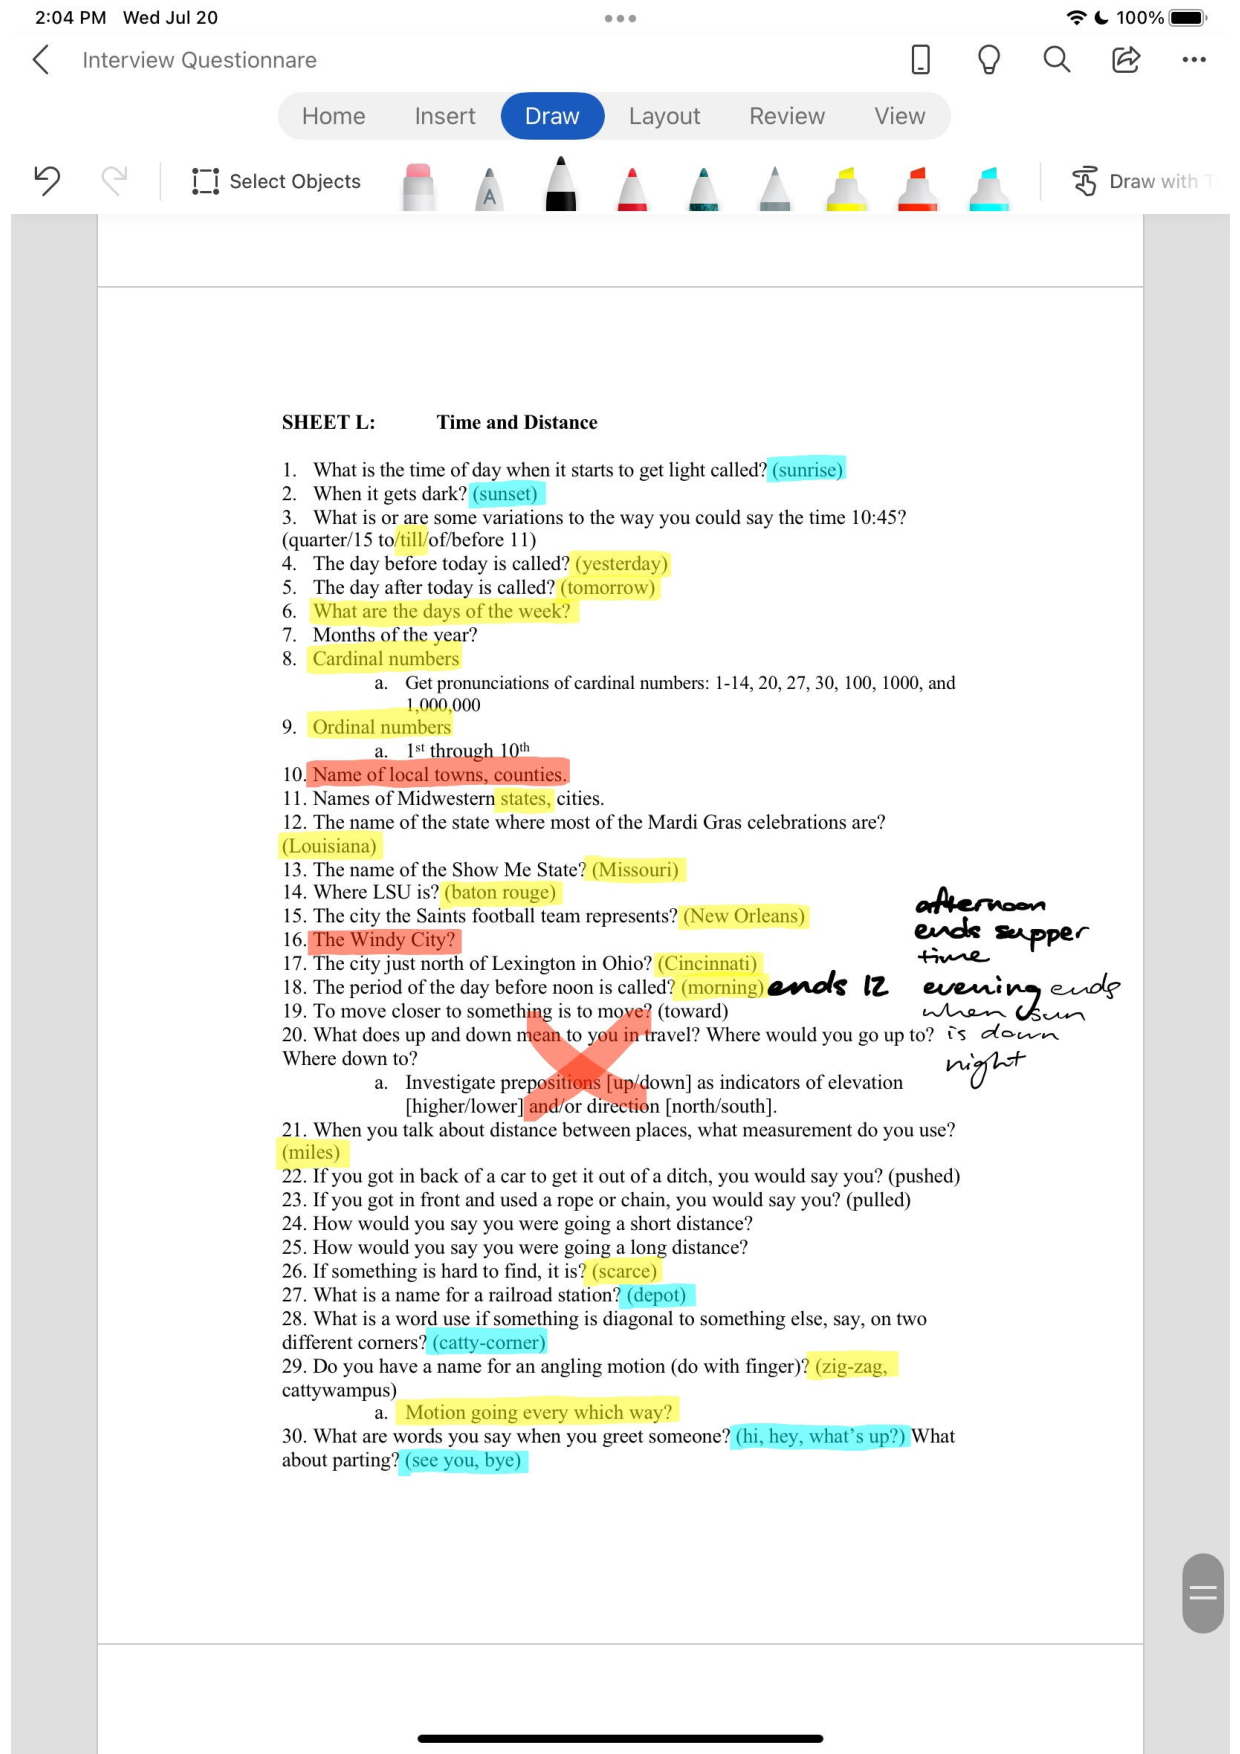
\includegraphics[width=\textwidth]{burkette-img003b-color.pdf}
\end{minipage}%
\caption{\label{fig:burkette:3}Examples of student-generated digital notetaking during an LAP interview.}
\end{figure}
\vfill\pagebreak


With continued digitization efforts of older field records, recording, and notes, along with the use of the technologies we now have at our fingertips, we hope to bring the LAP into the 21\textsuperscript{st} century. 

\section{Conclusion} %5
\label{sec:burkette:5}
% \subsection{Closing remarks} %5.1

In this chapter, we have discussed current efforts to conduct new Atlas interviews in the state of Kentucky so that we can arrive at a better understanding of change and variation in the speech of the Bluegrass State. But also, we hope that we can encourage students looking for research topics (or who are just interested in the speech of the state in which they attend college) to consider adding to LAP coverage of the state. 

The method we have arrived at is informed by earlier LAP components, especially LAWS and LANCS, so that we can compare the results of new interviews to older LAP interviews. At the same time, we need to adapt, by tweaking worksheets so that we elicit the best data possible and by adopting newer technologies that create opportunities for analyzing our data in new and exciting ways.

We are also hoping that others will follow our lead and conduct interviews in other regions, states, and communities that were surveyed by earlier LAP components. Over the last several years, we have delved into the LAP archives and have digitized complete collections full of linguistic, cultural, and historical information that has not been properly tapped, such as the Linguistic Atlas of Hawaii and the Linguistic Atlas of the Pacific Northwest, as well as records from the Hudson Valley collected in the early 1940s. We are now nearing the point in this process that we can run investigations of linguistic features on the 5000-plus interviews in the LAP holdings, as evidenced by our recent paper on a-prefixing (\citealt{BurketteAntieau2022}), and we will soon be able to do this all online (Burkette forthcoming). The LAP represents a massive amount of time, energy, and effort -- on the part of fieldworkers, LAP office workers and administrators, as well as the speakers who gave of their time and community knowledge -- and our goal is to see that time appreciated through continued use of LAP materials and the expansion of contemporary LAP interviews.

\section*{Aknowledgements}

The authors would like to thank Dennis Preston, Jennifer Cramer, and Shane O’Nan for their contributions to this paper and this work. Thanks also to the two anonymous reviewers for their helpful suggestions. 

\sloppy\printbibliography[heading=subbibliography,notkeyword=this]
\end{document}
